\chapter{HIỂN THỊ KÝ TỰ TRÊN LCD} \label{Les:LCD}
\section{Giới thiệu chung}
\subsection{Yêu cầu}
Viết chương trình hiển thị ký tự lên LCD.
\subsection{LCD}
Chức năng các chân của LCD:
\begin{table}[!h]
\begin{center}
\begin{longtable}{|c|c|p{5cm}|p{4.5cm}|l}\cline{1-4}
\textbf{STT} & \textbf{Ký hiệu} & \centering{\textbf{Mô tả}} & \centering{\textbf{Giá trị}} & \\ \cline{1-4}
1 & VSS & GND & $0V$ & \\ \cline{1-4}
2 & VCC & & $5V$ & \\ \cline{1-4}
3 & VEE & Tùy chỉnh độ tương phản & & \\ \cline{1-4}
\multirow{2}{.5cm}{ 4} & \multirow{2}{.8cm}{RS} & \multirow{2}{5cm}{Lựa chọn thanh ghi} & RS = 0: ghi lệnh & \\
& & & RS = 1: ghi dữ liệu & \\ \cline{1-4}
\multirow{2}{.5cm}{5} & \multirow{2}{.8cm}{R/W} & \multirow{2}{5cm}{Chọn thanh ghi đọc/viết dữ liệu} & R/W = 0: viết dữ liệu & \\
& & & R/W = 1: đọc dữ liệu & \\ \cline{1-4}
6 & E & Enable & & \\ \cline{1-4}
$7-10$ & DB0 -- BD3 & \multirow{2}{5cm}{Chân chuyền dữ liệu} & \multirow{2}{5cm}{8 bit từ $DB0 \rightarrow DB7$} & \\ 
$11-14$ & DB4 -- DB7 &  & & \\ \cline{1-4} 
%9 & DB2 &  & & \\  
%10 & DB3 &  & & \\  
%11 & DB4 &  & & \\  
%12 & DB5 &  & & \\  
%13 & DB6 &  & & \\  
%14 & DB7 &  & & \\ \cline{1-4}
15 & A & Cực dương của LED nền & $0 - 5V$& \\ \cline{1-4}
16 & K & Cực âm của LED nền & $0V$ & \\ \cline{1-4}
\end{longtable}
\end{center}
\caption{Sơ đồ chân và chứa năng các chân của LCD}
\label{Fig:lcd}
\end{table}
%\newpage

Ngoài sử dụng LCD, người ta còn sử dụng các LED 7 đoạn, LED ma trận để hiển thị dữ liệu (với LED 7 đoạn có trong \textit{phụ lục \ref{app:led-7-doan} trang \pageref{app:led-7-doan}}).
\subsection{Sơ đồ mạch}
\begin{figure}[!h]
\begin{center}
%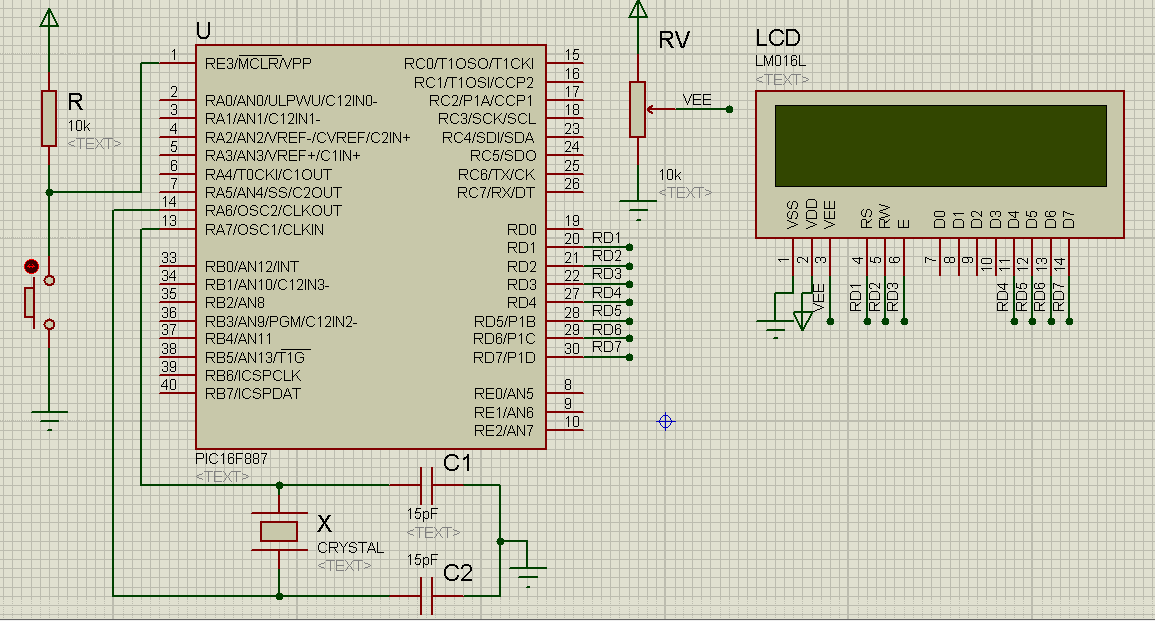
\includegraphics[width=3cm, height=4cm]{bai-2/image/BAI-2}
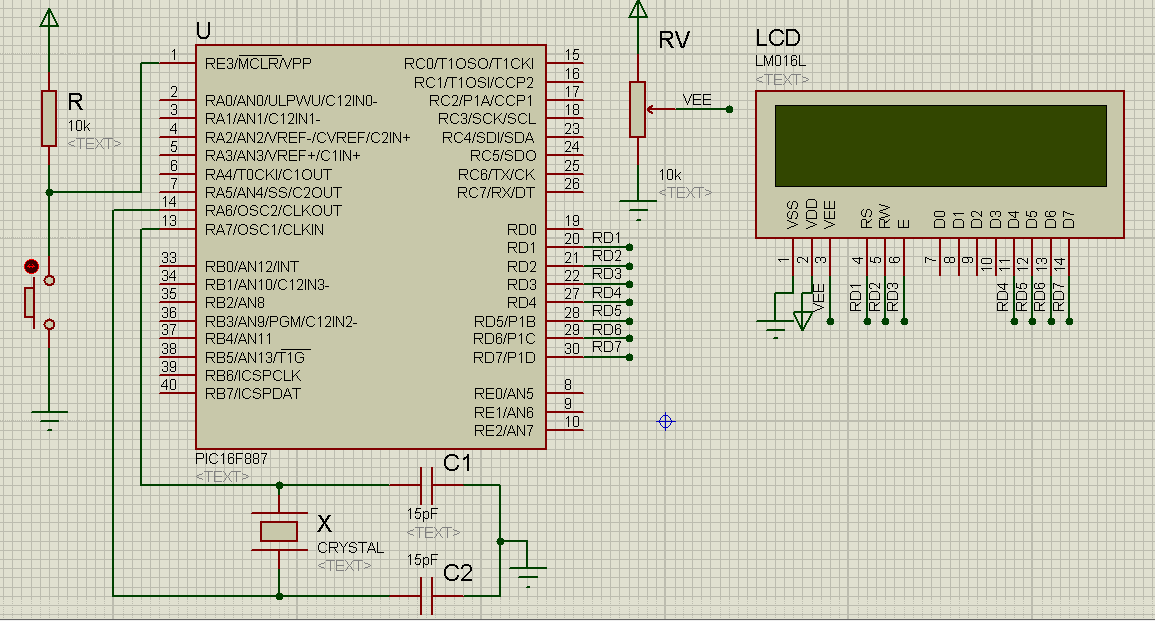
\includegraphics[scale=0.5]{bai-2/image/BAI-2}
\end{center}
\caption{Mạch điều khiển LCD}
\end{figure}
\section{Sử dụng các lệnh cơ bản cho LCD}
Sử dụng thư viện \verb|LCD_LIB_4BIT.C| (trong \emph{phụ lục trang \pageref{def:lcd}}) để điều khiển LCD.

Các bước cơ bản đề bắt đầu làm việc với LCD:
\begin{itemize}
\item Thêm thư viện LCD vào chương trình: \verb|#include<LCD_LIB_4BIT.C>|
\item Chúng ta dùng LCD ở chế độ ghi, dùng lệnh: \verb|OUTPUT_LOW(LCD_RW);| (trong \emph{bảng \ref{Fig:lcd} trang \pageref{Fig:lcd}}).
\item Khởi tạo LCD, dùng hàm: \verb|LCD_Init();|
\item Chức năng của một số hàm có trong thư viện được sử dụng:
\begin{itemize}
\item Hàm \verb|LCD_Init();| Khởi tạo LCD.
\item Hàm \verb|LCD_PutCmd(unsinged int cX);| Gửi lệnh lên LCD.

Ví dụ: \verb|LCD_PutCmd(0x01);| -- lệnh xóa màn hình.
\item Hàm \verb|LCD_PutChar(unsinged int cX);| Ghi một chuỗi hoặc một ký tự lên LCD.
\item Hàm \verb|LCD_SetPosition(unsinged int cX);| Thiết lập vị trí con trỏ.
\begin{itemize}
\item Dòng 1: bắt đầu từ vị trí \verb|0x00|, tăng giá trị này lên để đến các vị trí khác trên dòng 1.
\item Dòng 2: bắt đầu từ vị trí \verb|0x40|, tăng giá trị này lên để đến các vị trí khác trên dòng 2.
\end{itemize}
\end{itemize}
\item Cách sử dụng hàm \verb|printf(tham số)|: 
\begin{itemize}
\item Xuất chuỗi, ký tự: \verb|printf("Chuỗi, ký tự cần xuất");|
\item Xuất số nguyên: \verb|printf("N = %d",n);| số nguyên ngắn dùng \verb|%d|, số nguyên dài dùng \verb|%lu|
\item Xuất số thực: \verb|printf("A = %.2f",a);| quy định số chữ số sau dấy phẩy (trong ví dụ: quy định $2$ chữ số sau dấu phẩy).
\end{itemize}
\item Các cấu trúc: \verb|while, for, if, if...else,|\ldots
\end{itemize}
\section{Bài tập}
\subsection{Bài tập 2.1}
\paragraph{Yêu cầu}Viết chương trình hiển thị các ký tự sau lên LCD: \verb|DAI HOC KTCN CAN THO|
\paragraph{Hướng giải quyết}
\begin{itemize}
\item Thiết lập LCD ở chế độ ghi: \verb|OUTPUT_LOW(LCD_RW);|
\item Khởi tạo LCD: \verb|LCD_Init();|
\item Xóa màn hình: \verb|LCD_PutCmd(0x01);|
\item Ghi ký tự lên LCD:
\begin{itemize}
\item Cài đặt vị trí con trỏ: ta chọn vị trí thứ 6 -- \verb|LCD_SetPosition(0x05);| để ghi chuỗi \verb|"DAI HOC"| trên dòng 1.

Chọn vị trí thứ 3 -- \verb|LCD_SetPosition(0x42);| để ghi chuỗi \verb|"KTCN CAN THO"| trên dòng 2.
\item Ghi chuỗi: \verb|LCD_PutChar("DAI HOC");| và \verb|LCD_PutChar("KTCN CAN THO");|
\end{itemize}
\end{itemize}
\newpage
\section*{Kết quả}
\begin{figure}[!h]
%\vspace{-.5cm}
\begin{center}
  {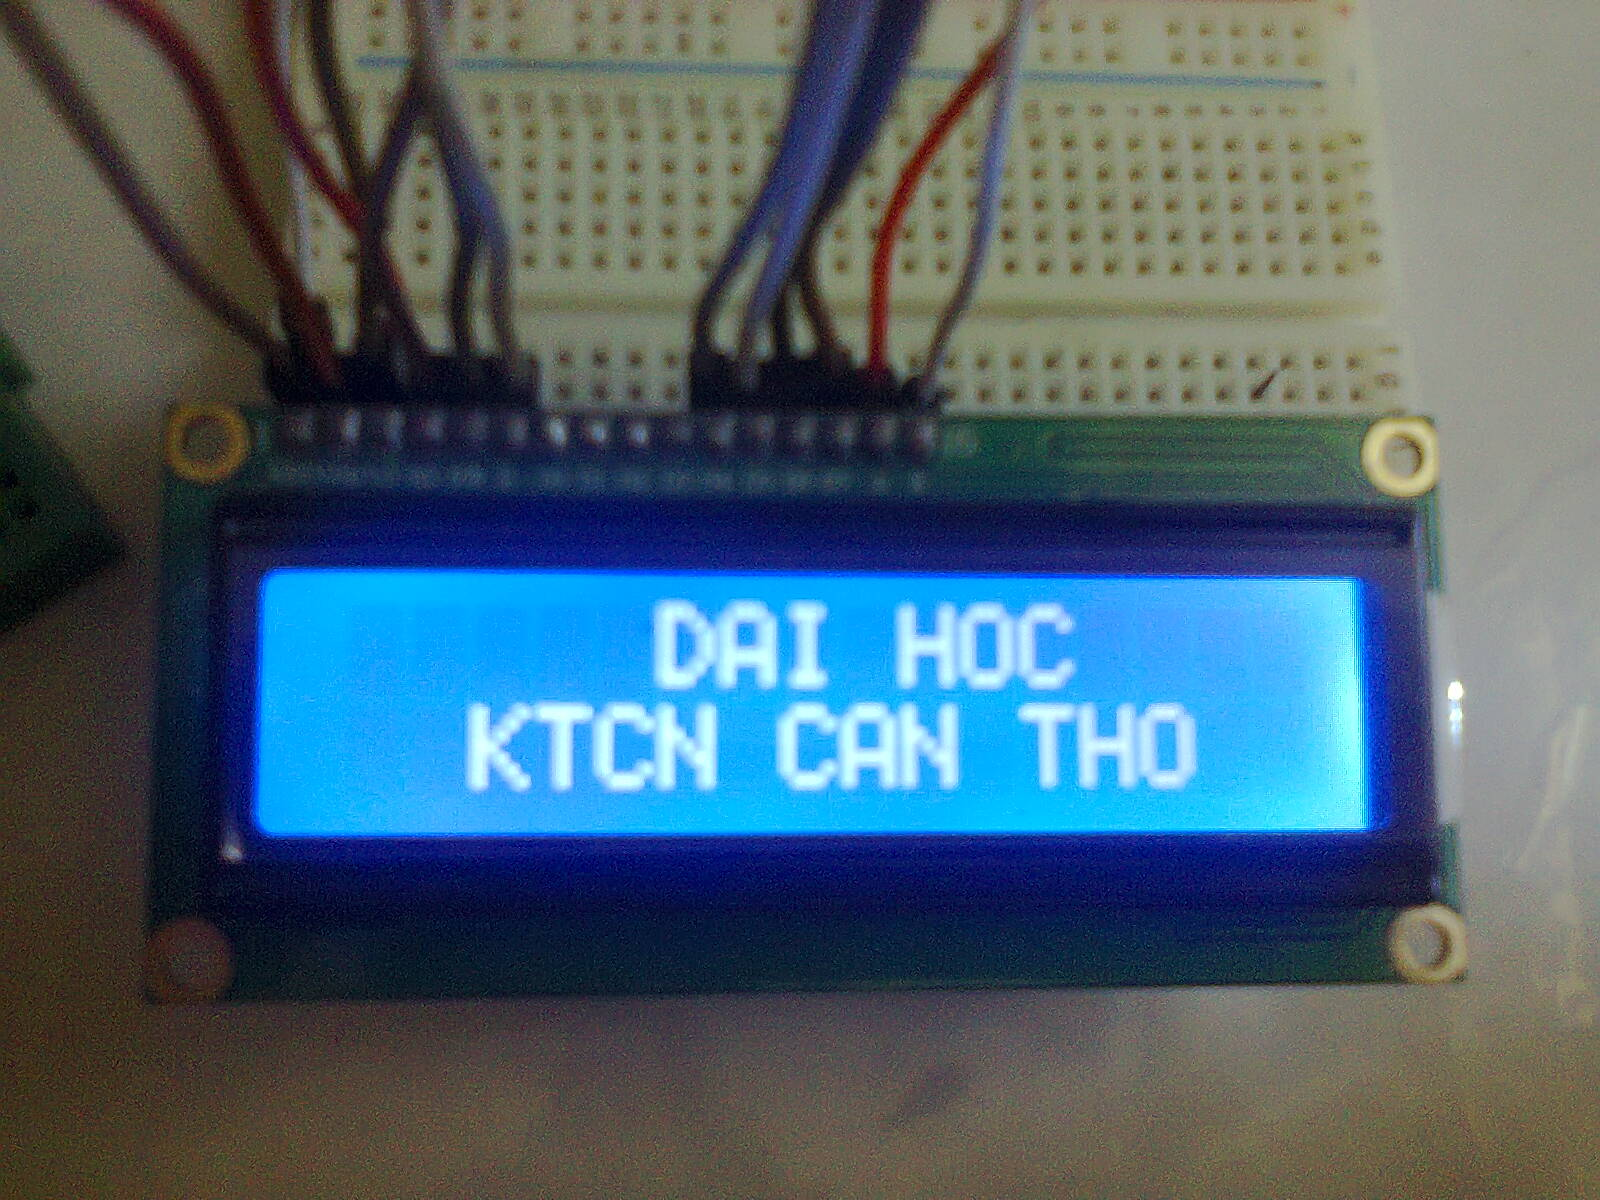
\includegraphics[width=.5\linewidth]{bai-2/image/2-1}}
\end{center}
\caption{Kết quả hiển thị ký tự lên LCD 16x02}
\end{figure}
\subsection*{Chương trình 4}
\lstinputlisting[language=C]{BAI-2-1.C}
\subsection{Bài tập 2.2}
\paragraph{Yêu cầu}Viết chương trình hiển thị trên \verb|LCD| theo yêu cầu sau: Hàng thứ nhất hiển thị họ tên sinh viên; hàng thứ hai hiển thị mã số sinh viên.
\paragraph{Hướng giải quyết}Sử dụng lại \emph{chương trình 4} của \emph{bải tập 2.1} với các thay đổi: vị trí con trỏ và chuỗi ký tự để phù hợp với yêu cầu.
\subsection*{Kết quả}
\begin{figure}[!h]
\begin{center}
  {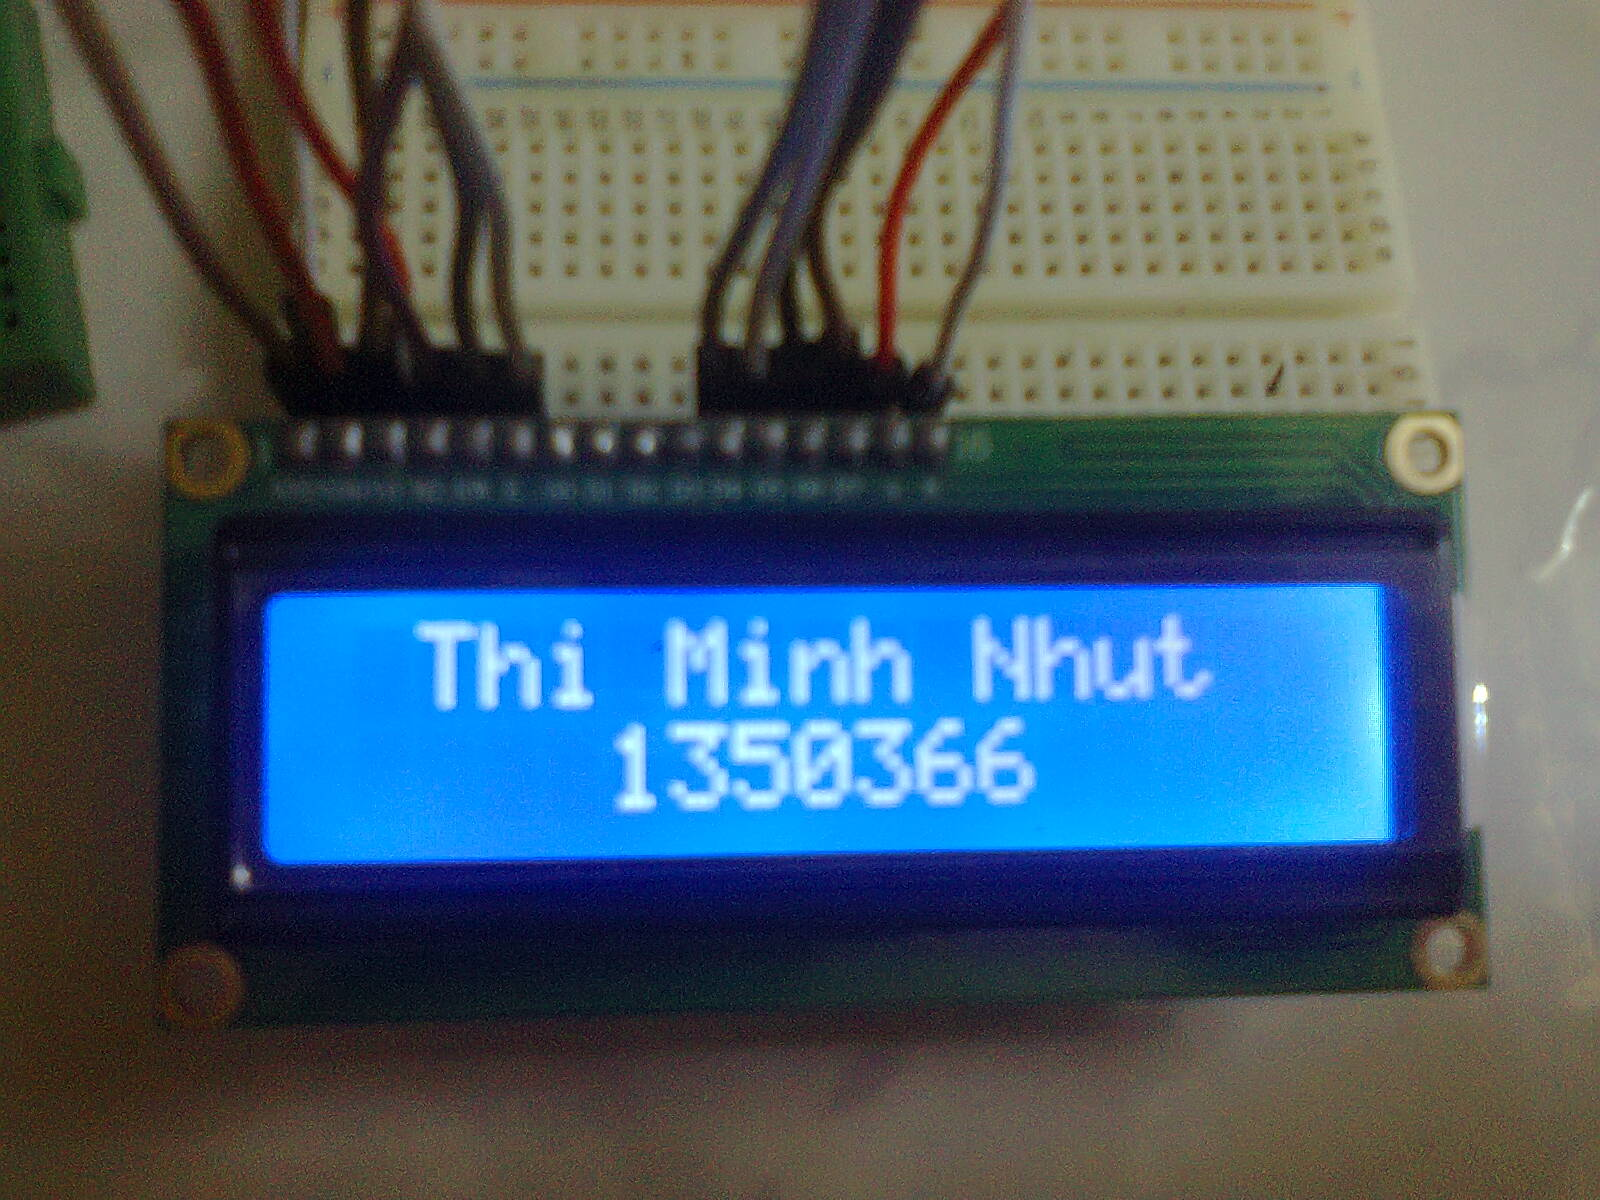
\includegraphics[width=.5\linewidth]{bai-2/image/2-2}}
\end{center}
\caption[]{Kết quả hiển thị họ tên và mã số sinh viên lên LCD 16x02}
\end{figure}
\subsection*{Chương trình 5}
\lstinputlisting[language=C]{BAI-2-2.C}
\subsection{Bài tập 2.3}
\paragraph{Yêu cầu}Viết chương trình đếm số từ $0$ đến $999$ hiển thị lên LCD.
\paragraph{Hướng giải quyết}
\begin{itemize}
\item Phần khai báo giống như \emph{bài tập 2.1}
\item Tăng giá trị số đếm: ban đầu ta gán biến đếm là \verb|count = 0;| rồi sử dụng cấu trúc \verb|for| để tăng giá trị biến đếm lên (\verb|count++;|)
\item Do cần hiển thị số lên LCD nên ta dùng hàm \verb|LCD_PutChar| kết hợp với hàm \verb|printf| để làm việc này.
\begin{itemize}
\item Hiển thị số nguyên: ví dụ \verb|unsigned long n = 12345| thì dùng:

\verb|printf(LCD_PutChar,"%lu",n);|
\item Hiển thị số thực: ví dụ \verb|float n = 1.2345 | thì dùng:

\verb|printf(LCD_PutChar,"%.4f",n);|
\end{itemize}
\item Để hiển thị giá trị biến đếm lên LCD, dùng:

\verb|printf(LCD_PutChar,"%lu",count);|

khi \verb|count| vượt quá giá trị, đưa biến \verb|count = 0;|
\end{itemize}
\subsection*{Kết quả}
\begin{figure}[!h]
\begin{center}
  {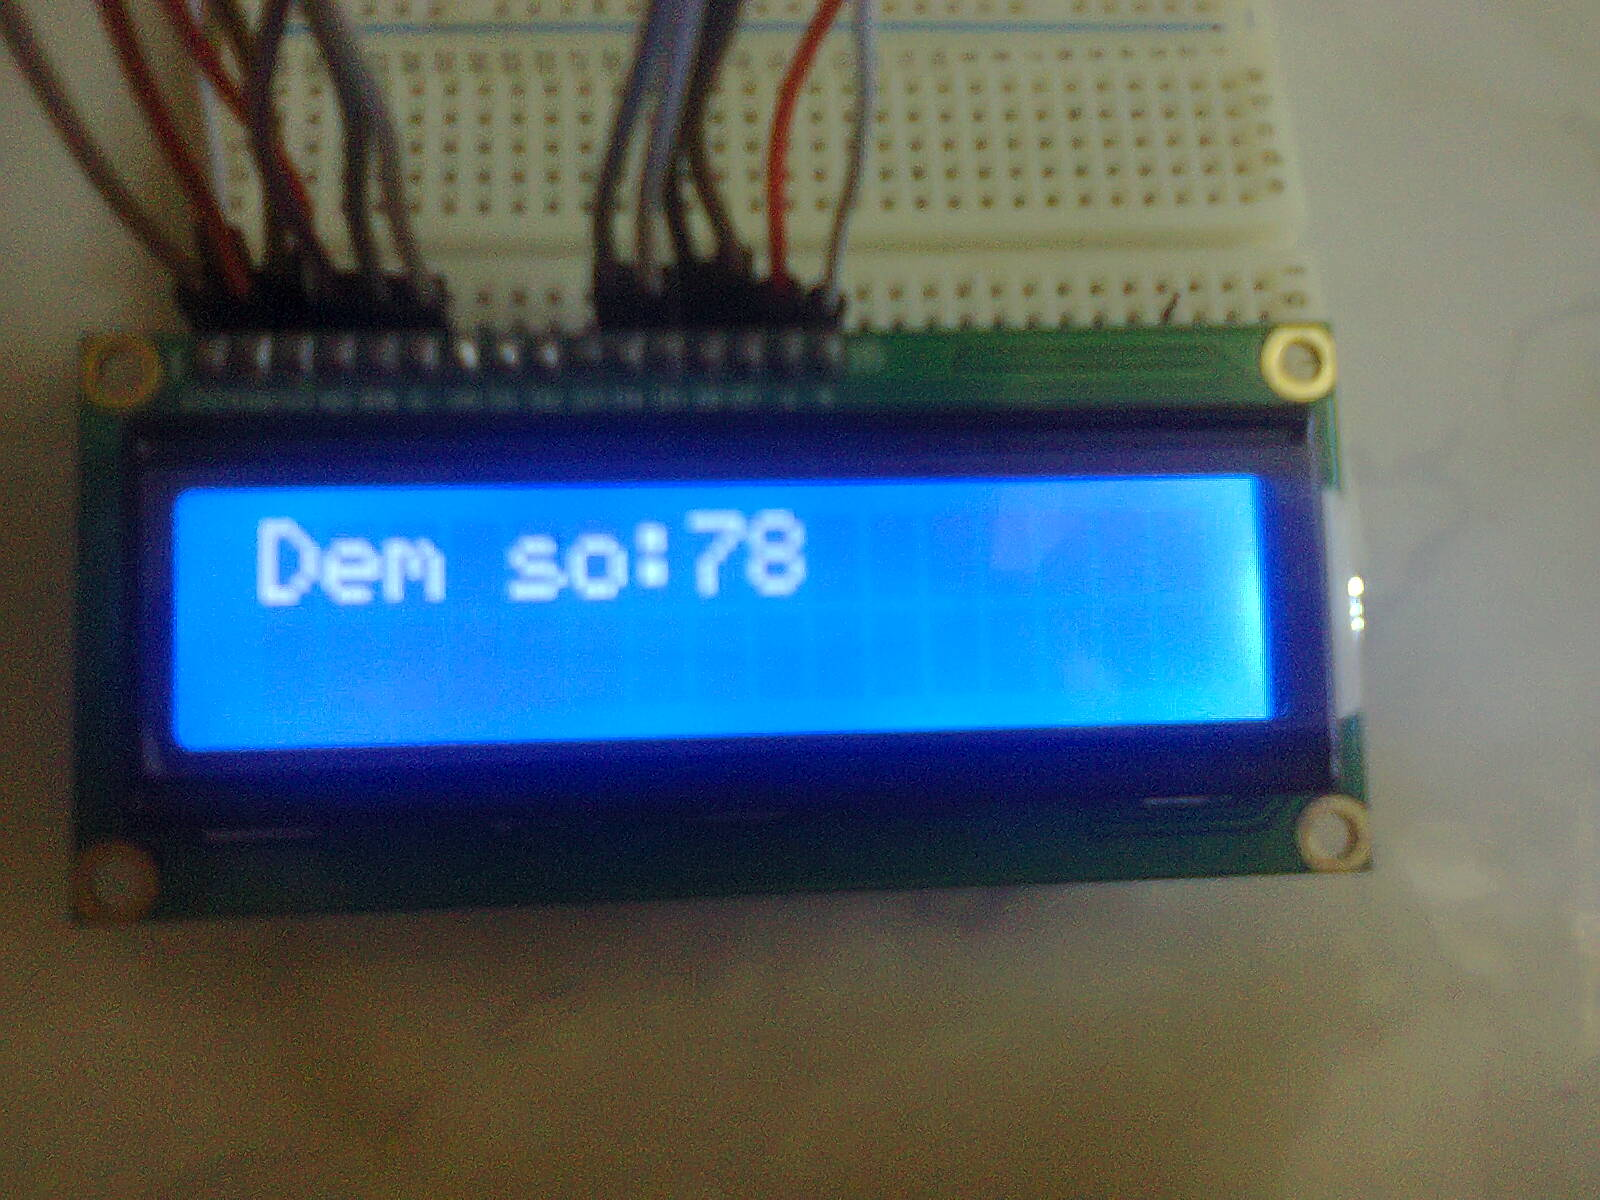
\includegraphics[width=.3\linewidth]{bai-2/image/2-3}}
\end{center}
\caption[]{Kết quả chương trình đếm số hiển thị lên LCD 16x02}
\end{figure}
\subsection*{Chương trình 6}
\lstinputlisting[language=C]{BAI-2-3.C}